
%(BEGIN_QUESTION)
% Copyright 2011, Tony R. Kuphaldt, released under the Creative Commons Attribution License (v 1.0)
% This means you may do almost anything with this work of mine, so long as you give me proper credit

This control system measures and regulates the differential pressure across a large motor-driven gas compressor by ``recycling'' gas from the compressor's discharge line back to its suction line.  It uses an air-to-close control valve so that the valve will fail open in the event of air pressure or signal loss.  The controller's output indication, however, is reverse-responding so that 0\% (20 mA) represents a fully shut valve while 100\% (4 mA) represents a wide-open valve:

$$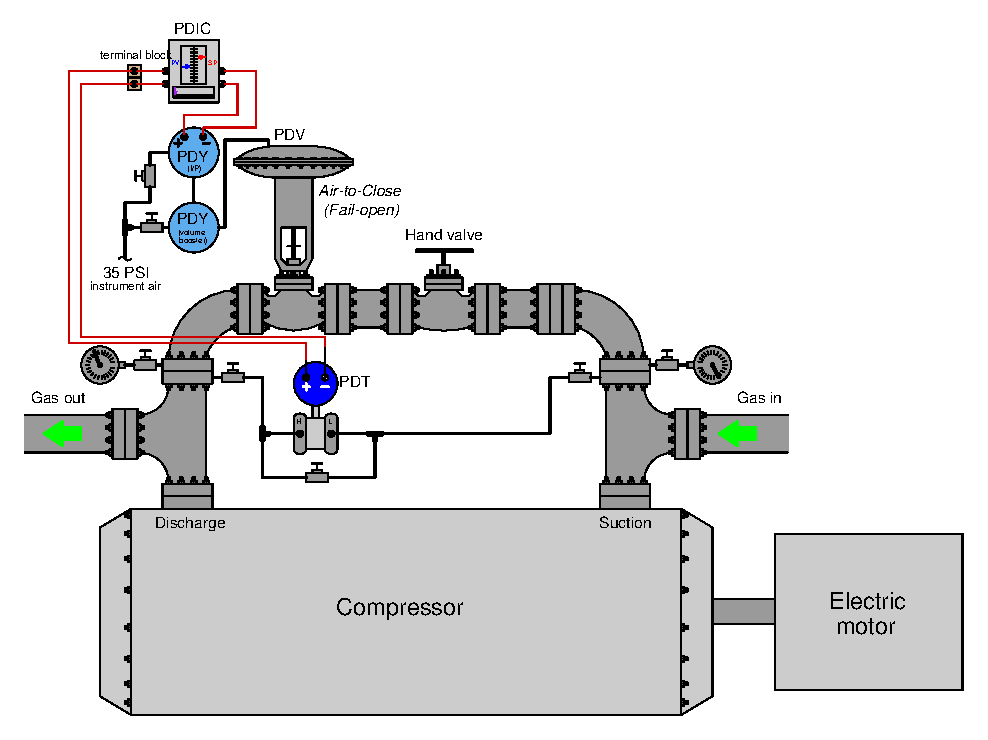
\includegraphics[width=15.5cm]{i00294x01.eps}$$

Unfortunately, this system has a problem.  The pressure differential indicating controller (PDIC) shows the process variable (PV) being about 50\% of range, while the setpoint (SP) is adjusted to 70\%.  The controller's output indication shows 0\%.

Identify which of these four areas of the system the problem may be located in, and then describe a good test you could do in or to this system to narrow the problem location even further:

\begin{itemize}
\item{} Problem with the measurement side (transmitter, wiring, controller analog input)?
\item{} Problem with the controller's control action (its ``decision-making'')?
\item{} Problem with the final control element side (valve, I/P, booster, controller analog output)?
\item{} Problem with the compressor itself (or other portions of the process)?
\end{itemize}

\vskip 20pt \vbox{\hrule \hbox{\strut \vrule{} {\bf Suggestions for Socratic discussion} \vrule} \hrule}

\begin{itemize}
\item{} Could a shut recycle line hand valve account for what we're seeing here?  Explain why or why not.
\end{itemize}

\underbar{file i00294}
%(END_QUESTION)





%(BEGIN_ANSWER)

The problem is clearly {\it not} with the controller's action, because according to the faceplate displays it is trying to do the right thing (i.e. shut the control valve to build up differential pressure).

%(END_ANSWER)





%(BEGIN_NOTES)

The measurement side of the system may be falsely registering a low pressure (i.e. the pressure is actually greater than what the controller shows), or the valve is opening when it should not (i.e. it is causing the differential pressure to be this low), or the compressor may be performing poorly and not be able to raise the required differential pressure, or the larger process may be drawing too heavily on the compressor.

\vskip 10pt

A good test would be to see whether the differential pressure is actually as low as the controller shows.  Another test would be to see whether the control valve is actually open when it should be shut.  Using a milliammeter to measure either PV or output signal (mA) would be an excellent place to begin, to verify the controller's I/O signals and check for correspondence between the controller's display and the signals.

%INDEX% Basics, control loop troubleshooting: isolating area of fault by correspondence
%INDEX% Process: compressor differential pressure control
%INDEX% Process: compressor surge control

%(END_NOTES)


